% Chapter Template

\chapter{Introduction to Machine Learning} % Main chapter title

\label{ChapterIntroML}


\section{Basic Concepts of Machine Learning}
Machine Learning (ML) is a field of computer science that groups a variety of  methods whose aim is giving computers the ability of \emph{learning}. The more cited definition of \emph{learning} has been provided by Mitchell in 1997 \cite{Mitchell1997}: \enquote{ A computer program is said to learn from experience E with respect to some task T and performance measure P, if its performance on T, as measured by P, improves with experience E.} \\
The ML methods methods essentially come from applied statistics, and are characterised by an increased emphasis on the use of computers to statistically estimate complicated functions. This allows ML to tackle tasks that would be too difficult to solve with algorithms entirely designed and specified by human being. An ML algorithm is often said to \enquote{learn from data}, in the sense that it is able to improve an algorithm's performance at some task via a data observation experience.

\subsection{The Task, the Performance and the Experience}\label{sec:TPE}
\paragraph*{The task.} The task T is usually described in terms of how the ML system should process an \emph{example} (or \emph{data point}). An \emph{example} is one datum $\vLeakVec\in \mathbb{R}^\traceLength$, which is in turn a collection of \emph{features} $\vLeakVec[i]$, with  $i=1,\dots \traceLength$. In SCA context an example might be a side-channel trace, which is in turn a collection of time samples, that constitute its features. Some common ML tasks include these three examples: 
\begin{itemize}
\item \emph{Regression: } the computer is asked to approximate a mapping function from some input variables to some continuous output variables, \eg approximate $\MLmodel\colon \mathbb{R}^\traceLength \rightarrow \mathbb{R}$.
\item \emph{Classification: } the computer is asked to specify which class or category an input belongs to, being $\sensVarSet$ the set of the possible classes. The learning algorithm is thus asked to construct a function $\MLmodel\colon \mathbb{R}^\traceLength \rightarrow \sensVarSet$. We remark that this task is similar to the regression one, except for the form of the output, since in general $\sensVarSet$ is a discrete finite set, and not continuous. A slightly variant solution to the classification task consists in constructing a function $\MLmodel\colon \mathbb{R}^\traceLength \rightarrow \{0,1\}^{\numClasses}$, if elements of $\sensVarSet$ are expressed \via the \emph{one-hot encoding} (see \ref{sec:notations}). Another variant of the classification task consists in finding a function $\MLmodel$ defining a probability distribution over classes.
\item \emph{Verification}: the computer is asked to state whether or not two given inputs are instances of a same class or category. For example, it may be asked to state if two hand-written signatures have been produced by the same person. The learning algorithm is thus asked to construct a function $\MLmodel\colon \mathbb{R}^\traceLength \times \mathbb{R}^{\traceLength}\rightarrow \{0,1\}$. A variant of such a task consists in finding a function $\MLmodel$ defining the probability of each pair of inputs being instances of a same class. 
\end{itemize}
The functions constructed by an ML algorithm somehow describe and characterise the data form and distribution, thus are often referred to as \emph{models}.

\paragraph*{The performance measure.} The performance measure P designs a quantification of the ability of the learning algorithm. Depending on the task T, a specific performance measure P can be considered. For tasks as classification or verification the more common measure is the \emph{accuracy} of the model, \ie the proportion of inputs for which the model produces the correct output. Equivalently, the \emph{error rate} may be used as a performance measure P, \ie the proportion of inputs for which the model produces an incorrect output. For the regression task the more common performance measure P is the so-called \emph{Mean Squared Error} (MSE): it is computed by averaging over a finite set of examples, the squares of the the differences between the correct outputs and the ones predicted by the model.\\
One of the crucial challenges of ML is that we are usually interested in how well a learning algorithm performs in producing a model that fits new, unseen data. For this reason, the performances of an ML algorithm are usually evaluated over a so-called \emph{test set}, \ie a set of examples that have not been used for the learning (or \emph{training}) phase. 

\paragraph*{The experience.} The experience E describes the way data and information are accessed by the learning algorithm during learning. In this context we principally distinguish two families of learning algorithms: 
\begin{itemize}
\item the \emph{supervised} learning algorithms access to a dataset of examples, each associated in general to a \emph{target} or \emph{label}. The term supervised reflects the fact that the learning is somehow guided by an instructor that knows the right answer over the learning dataset;
\item the \emph{unsupervised} learning algorithms access to a dataset, without any associated target. They try to learn useful properties of the structure of the dataset. 
\end{itemize}
In general, the nature of the task is strictly related to the kind of experience the learner is allowed; for example the classification or regression tasks are considered as supervised tasks, while examples of unsupervised tasks include \emph{clustering} and \emph{data representation} or \emph{dimensionality reduction}. For example, the Principal Component Analysis, that will be discussed in Chapter~\ref{ChapterLinear} in the context of SCA, is a dimensionality reduction algorithm that might be seen as an unsupervised algorithm that learns a representation of data. We will see in Chapter~\ref{ChapterLinear} that for SCA context a supervised version of the PCA has been proposed as well. 


% examples: Classification, Dimensionality Reduction, Verification
% Example method: Neural Network Classifier, Stacked Auto-Encoder, Siamese Network 

\subsection{Example of Linear Regression}
The regression task is not of high interest for the rest of this thesis, but is the most direct example to keep in mind in order to understand some basic ML concepts, such as the \emph{underfitting} and the \emph{overfitting} (see \ref{sec:overfitting}). Let us introduce a linear regression model to tackle the regression task: we want to construct a linear function $\MLmodel\colon \mathbb{R}^\traceLength \rightarrow \mathbb{R}$, that takes an input $\vLeakVec$ and outputs $\hat{y} = \www^\intercal \vLeakVec$, where $\www\in \mathbb{R}^\traceLength$ is a vector of \emph{parameters} that have to be learned by a learning algorithm in order to well describe some data.\footnote{An affine model may be considered as well by adding a \emph{bias}, leading to $\hat{y} = \www^\intercal \vLeakVec+w_0$. This model is equivalently obtained by adding an additional component to $\vLeakVec$, always set to $1$ and by writing back $\hat{y} = \www^\intercal \vLeakVec$ with $\www\in \mathbb{R}^{\traceLength+1}$. } 
Let $\setData_{\cdot} = (\setLeak_{\cdot}, \setTarget_{\cdot})$ denote a dataset, where $\cdot$ can stand for \textquotedbl$\text{train}$\textquotedbl \ or \textquotedbl$\text{test}$\textquotedbl \ depending on the role of the dataset in the experience, and let $\sizeSetData$ denote the size of the dataset, \ie the number of examples contained in it. Let us store the examples contained in $\setLeak_{\cdot}$ into a matrix $\measuresMatrix_{\cdot}\in \mathbb{R}^{\traceLength \times \sizeSetData}$ and the targets contained in $\setTarget_{\cdot}$ into a targets vector $\yyy_{\cdot}\in \mathbb{R}^{\sizeSetData}$. Let a learned model predict targets $y_i$ by outputting $\hat{y_i} = \www^\intercal\vLeakVec_i$ and let them be collected in turn into a predicted targets vector $\hat{\yyy}_{\cdot}$. The MSE is given by 

\begin{equation}
 \mathrm{MSE_{\cdot}} = \frac{1}{\sizeSetData} \norm{\hat{\yyy}_{\cdot}-\yyy_{\cdot}}^2_2 \mbox{ .}
\end{equation}

The performance measure for the learning algorithm is $\mathrm{MSE_{test}}$, meaning that the goal for the learning algorithm is to find a parameter vector $\www$ which minimises $\mathrm{MSE_{test}}$. Nevertheless, such an objective cannot be directly imposed, because the learning algorithm only experiences over the training set, and not over the test set. An intuitive way to act, that can be proven to be the maximum-likelihood solution to the problem, is to minimise  $\mathrm{MSE_{train}}$ instead of $\mathrm{MSE_{test}}$. This minimization can be obtained by solving an easy optimization problem. When a learning algorithm behaves as an optimization algorithm that minimises a given function, such a function is called \emph{cost function}, or \emph{loss function}, or \emph{objective function}. 
The solution to such an optimization problem can be given in closed form, by means of the \emph{pseudo-inverse} matrix $\measuresMatrix^+$ of $\measuresMatrix_{\text{train}}$, as follows:
\begin{equation}
\measuresMatrix^+ = (\measuresMatrix_{\text{train}}\measuresMatrix_{\text{train}}^\intercal)^{-1}\measuresMatrix_{\text{train}}
\end{equation}
\begin{equation}
\www = \measuresMatrix^+\yyy_{\text{train}}.
\end{equation}

%OLD 
%We want this model well describe some data and we suppose to have two available datasets of such data: $\setDataTrain = (\setLeakTrain, \setTargetTrain)$, to let the learning algorithm experience on, and $\setDataTest = (\setLeakTest, \setTargetTest)$ to evaluate its performance over some unseen data. Let us choose the MSE over the test set to evaluate such performances. Let us collect the examples $(\vLeakVec_i, y_i)_{i=1,\dots, N}$ of a dataset into a measure matrix $\measuresMatrix_{\text{train}}\in \mathbb{R}^{\traceLength \times N}$ and into a targets vector $\yyy_{\text{train}}\in \mathbb{R}^N$ (or $\yyy_\text{test}$ for the test dataset), and let the learned model predict targets $y_i$ by outputting $\hat{y_i} = \www^\intercal\vLeakVec_i$ (in turn collected into a predicted targets vector $\hat{\yyy}_{\text{train}}$, or $\hat{\yyy}_{\text{test}}$ if working with the test dataset), then the MSE is given by
%\begin{equation}
% \mathrm{MSE_{test}} = \frac{1}{m} \norm{\hat{\yyy}_{\text{test}}-\yyy_{\text{test}}}^2_2 \mbox{ .}
%\end{equation}
%Obviously, we consider the model performs well the most such an MSE is small. So the goal of the learning algorithm is to somehow minimize the $\mathrm{MSE_{test}}$. But the learning algorithm only experiences on the $\setDataTrain$ dataset. An intuitive way to act, that can be proven to be the maximum likelihood solution to the problem, is to minimize  $\mathrm{MSE_{train}}$ instead of $\mathrm{MSE_{test}}$. This minimization can be obtained by solving an easy optimization problem. When a learning algorithm behaves as an optimization algorithm that minimizes a given function, such a function is called \emph{cost function}, or \emph{objective function}.
% The solution to such an optimization problem can be given in closed form, by means of the pseudo-inverse matrix of $\measuresMatrix_{\text{train}}$:
%\begin{equation}
%\www = (\measuresMatrix_{\text{train}}\measuresMatrix_{\text{train}}^\intercal)^{-1}\measuresMatrix_{\text{train}}\yyy_{\text{train}}.
%\end{equation}


\subsection{Example of Linear Model for Classification}\label{example:LDA}
As observed in Sections \ref{sec:simple} and \ref{sec:advanced}, a strict relationship may be established between the profiling SCAs and the classification task in ML context. For this reason we introduce here a very brief overview of how classically the classification task is tackled, by means of linear models. \\
Classifying means assigning a label $\sensVar\in \sensVarSet$ to an example $\vLeakVec\in\mathbb{R}^\traceLength$ , or equivalently divide the input space $\mathbb{R}^\traceLength$ in \emph{decision regions}, whose boundaries are referred to as \emph{decision boundaries}. Making use of a linear model signifies exploiting some hyperplanes as decision boundaries. Datasets whose classes can be separated exactly by linear decision boundaries are said to be \emph{linearly separable}. Following the discussion kept by Bishop in \cite{christopher2006pattern}, two different approaches to tackle the classification task should be distinguished: the direct research for a discriminant function $\MLmodel$ that assigns to an example a label, or the prior construction of a probabilistic model. This second approach might in turn be distinguished into two options, depending on whether a \emph{generative} model  (see Sec.~\ref{sec:TA}), or a \emph{discriminative} model is constructed (\ie only conditional probability densities of outputs given the inputs are modelled). For this example we consider a probabilistic approach, constructing a generative model, which is the same approach of Template Attacks (Sec.~\ref{sec:TA}). This example will allow on one hand to introduce some interesting functions, such as the \emph{logistic sigmoid} and the \emph{softmax}, that will play a role in the construction of Neural Networks (see Chapter \ref{ChapterCNN}). On the other hand, the example justifies the large exploitations of generalised linear models in order to construct discriminative functions. Indeed, linear models come out naturally when adding some assumptions on the data distributions, as those that will be introduced below. \\

Constructing a generative probabilistic model implies modelling the class-conditional probabilities $\pdf_{\given{\vaLeakVec}{\sensRandVar = \sensVarValue{j}}}(\vLeakVec)$ for $j\in \{1,\dots,\numClasses\}$ as well as the class priors $\pdf_{\sensRandVar}(\sensVarValue{j})$ and $\pdf_{\vaLeakVec}(\vLeakVec)$. Let us first consider a 2-class context, \ie $\sensVarSet = \{\sensVarValue{1}, \sensVarValue{2}\}$. Then, the posterior probability for the class $\sensVarValue{1}$ is the following:
\begin{align}\label{eq:post_probs}
\prob(\given{\sensVarValue{1}}{\vLeakVec}) &= \frac{\prob(\given{\vLeakVec}{\sensVarValue{1}})\prob(\sensVarValue{1})}{\prob(\vLeakVec)}=\\
&=\frac{\prob(\given{\vLeakVec}{\sensVarValue{1}})\prob(\sensVarValue{1})}{\prob(\given{\vLeakVec}{\sensVarValue{1}})\prob(\sensVarValue{1}) + \prob(\given{\vLeakVec}{\sensVarValue{2}})\prob(\sensVarValue{2})}\mbox{ .}
\end{align}
To compare the two classes, we can evaluate their \emph{log-likelihood ratio} defined as:
\begin{equation}\label{eq:log-ratio}
a = \log\left[\frac{\prob(\given{\sensVarValue{1}}{\vLeakVec})}{\prob(\given{\sensVarValue{2}}{\vLeakVec})}\right] =  \log\left[\frac{\prob(\given{\vLeakVec}{\sensVarValue{1}})\prob(\sensVarValue{1})}{\prob(\given{\vLeakVec}{\sensVarValue{2}})\prob(\sensVarValue{2})}\right].
\end{equation}
Then we might assign the label the class $\sensVarValue{1}$ to $\vLeakVec$  if and only if $a>0$, which corresponds to take as decision boundary the surface defined by $\prob(\given{\vLeakVec}{\sensVarValue{1}})\prob(\sensVarValue{1}) = \prob(\given{\vLeakVec}{\sensVarValue{2}})\prob(\sensVarValue{2})$.
We remark that Eq.~\eqref{eq:post_probs} rewrites as:
\begin{equation}\label{eq:post_probs_sigmoid}
\prob(\given{\sensVarValue{1}}{\vLeakVec}) = \frac{1}{1+e^{-a}} = \sigma(a)\mbox{ ,}
\end{equation}
where the function $\sigma$ is the so-called \emph{logistic sigmoid}. This remark translates in the multi-class case, \ie $\numClasses >2$, in the following way: the posterior probability for each class $\sensVarValue{j}$ is given by
\begin{equation}\label{eq:post_probs_multi-class}
\prob(\given{\sensVarValue{j}}{\vLeakVec})  = \frac{\prob(\given{\vLeakVec}{\sensVarValue{j}})\prob(\sensVarValue{j})}{\prob(\vLeakVec)} = \frac{\prob(\given{\vLeakVec}{\sensVarValue{j}})\prob(\sensVarValue{j})}{\sum_{k=1}^{\nbClasses}\prob(\given{\vLeakVec}{\sensVar^k})\prob(\sensVar^k )} = \softmax (\aaa)[j]\mbox{ ,}
\end{equation}
where $\aaa$ is a $\numClasses$-dimensional vector, whose entries are given by
\begin{equation}\label{eq:softmax_entries}
\aaa[j] = \log\left[ \prob(\given{\vLeakVec}{\sensVarValue{j}})\prob(\sensVarValue{j}) \right] \mbox{ ,}
\end{equation}
and $\softmax$ is the so-called \emph{softmax} function, or \emph{normalised exponential}, that is defined, entry-wise by:
\begin{equation}\label{eq:softmax}
\softmax(\aaa)[k] = \frac{e^{\aaa[k]}}{\sum_{j=1}^{\numClasses}e^{\aaa[j]}}\mbox{ .}
\end{equation}

Let us now introduce two assumptions about the class-conditional densities:
\begin{enumerate}[label=(\roman*)]
\item \label{item:gaussian} we will suppose that they follow a Gaussian distribution with parameters $\mu_j, \Sigma_j$,
\item \label{item:covariances} and that all class-conditional densities share the same covariance matrix $\Sigma_j=\Sigma$,
\end{enumerate}
so that
\begin{equation}\label{eq:gauss_dens}
\pdf_{\given{\vaLeakVec}{\sensRandVar = \sensVarValue{j}}}(\vLeakVec)= \frac{1}{(2\pi)^{{\traceLength}/2}\lvert \Sigma\rvert^{1/2}}e^{-\frac{1}{2}(\vLeakVec- \mu_j)^\intercal\Sigma^{-1}(\vLeakVec- \mu_j)} \mbox{ .}
\end{equation}
Under these assumptions, and considering probability densities and masses instead of probability values\footnote{A formal justification of the validity of \eqref{eq:LDA-2classes} for continuous random variables is out of the scope of this section.} Eq.~\eqref{eq:log-ratio} rewrites as: 
\begin{equation}\label{eq:LDA-2classes}
a = \log\left[\frac{\pdf_{\sensRandVar}(\sensVarValue{1})}{\pdf_{\sensRandVar}(\sensVarValue{2})}\right] - \frac{1}{2}\mu_1^\intercal\Sigma^{-1}\mu_1 + \frac{1}{2}\mu_2^\intercal\Sigma^{-1}\mu_2 - \vLeakVec^\intercal\Sigma^{-1}(\mu_2-\mu_1) = \www^\intercal \vLeakVec + w_0, 
\end{equation}
where we set 
\begin{align*}
\www =& \Sigma^{-1}(\mu_1-\mu_2)\\
w_0 =  & \log\left[\frac{\pdf_{\sensRandVar}(\sensVarValue{1})}{\pdf_{\sensRandVar}(\sensVarValue{2})}\right] - \frac{1}{2}\mu_1^\intercal\Sigma^{-1}\mu_1 + \frac{1}{2}\mu_2^\intercal\Sigma^{-1}\mu_2 . 
\end{align*}
The quadratic terms in $\vLeakVec$, that appears in the exponent of the Gaussian density \eqref{eq:gauss_dens}, have cancelled thanks to the common variance assumption \ref{item:covariances}, thus we obtain that the decision boundary for the 2-class problem, given by $a=0$ is a $(\traceLength - 1)$-hyperplane of the input space.\footnote{An analogous result can be obtained in the multi-class problem.} This way of choosing linear boundaries is known under the name of \emph{Linear Discriminant Analysis}. Another way to view the same linear classification model is in terms of dimensionality reduction: intuitively, in the 2-class case\footnote{again extensible to the multi-class case} one can see the term $\www^\intercal \vLeakVec$ in \eqref{eq:LDA-2classes} as a projection of the input $\vLeakVec$ onto a one-dimensional subspace of $\mathbb{R}^\traceLength$ which is orthogonal to the decision boundary mentioned above. Then, the classification of the obtained dimensionality-reduced examples is done by the means of a real-valued threshold (that would correspond to $w_0$, in the optimal case). It can be shown that the dimensionality reduction obtained by the \emph{Fisher criterion} that we will deploy in Chapter~\ref{ChapterLinear}, to which we will refer to as LDA dimensionality reduction by a widely accepted abuse, is equivalent to the dimensionality reduction obtained in this example, under both assumptions \ref{item:gaussian} and \ref{item:covariances}.  \\
Relaxing the assumption \ref{item:covariances} and allowing each class-conditional density $\pdf(\vLeakVec\mid \sensVarValue{j})$ to have its own covariance matrix $\Sigma_j$, then the cancellations seen above will no longer occur, and the discriminant $a$ turns out to be a quadratic function of $\vLeakVec$. This gives rise to the so-called \emph{Quadratic Discriminant Analysis}, that we already mentioned in Chapter~\ref{ChapterIntroductionSCA} for its analogy with Template Attacks.\\

Assumptions \ref{item:gaussian} and \ref{item:covariances} also lead to the following expression for the posterior probability for $\sensVarValue{1}$, directly implied by \eqref{eq:post_probs_sigmoid}: 
\begin{equation}\label{eq:binary_linear_classifier}
\prob(\given{\sensVarValue{1}}{\vLeakVec}) = \sigma(\www^\intercal \vLeakVec + w_0)\mbox{ .}
\end{equation}
Thus, such a posterior probability is given by the sigmoid acting to a linear function of $\vLeakVec$. Similarly, for the multi-class case, the posterior probability of class $\sensVarValue{j}$ is given by the $j$-th entry of the softmax transformation of a linear function of $\vLeakVec$. This kind of \emph{generalised linear model} can be thus used in a probabilistic discriminant approach, where the posterior conditional probabilities are directly modelled from data without passing through the estimations of class-conditional densities and priors. Such a discriminative approach is the one that will be adopted in Chapter~\ref{ChapterCNN} when considering models constructed by Neural Networks.

%the simplest representations of a linear discriminant function is obtained by taking
%\begin{equation}
%f(\vLeakVec) = \www\vLeakVec + w_0 \mbox{ ,}
%\end{equation}
%where $-w_0$ plays the role of a threshold. Here  $\vLeakVec$ is assigned to $\sensVarValue{1}$ if $f(\vLeakVec)>0$, \ie $\www\vLeakVec>-w_0$, otherwise $\vLeakVec$ is assigned to $\sensVarValue{2}$.



% la decision boundary  è un D-1 iperpiano
% introducendo i vettori di target...
% y(x) = wx + w0...oppure in grosso per piu di due classi: la decision boundary è un iperpiano di dimensione (numClasses - 1)
% per imparare i pesi W un'idea è minimizzare il sum error square sti cazzi, un'altra è passare attraverso la riduzione di dimensione e scegliere la riduzione che amplifica la separabilità. 
%Infatti....fisher dà la nozione di ottimalità col quoziente, che porta alla Fisher Discriminant Analysis (o anche LDA, discussa nel Capitolo 6) ... Nel caso numClasses = 2 le due si equivalgono. 
% E interessante discutere brevemente anche di un semplice modello generativo, basato su hp gaussiana, perche tale ipotesi, insieme ad un'altra, porta a costruire anch'essa un modello lineare, giustificando questa scelta in molti contesti...P(x|C)...log del quoziente, funzione sigmoid, logit...softmax...linear piu sigmoid, dove di nuovo la soluzione LDA è la parte lineare (verifica). Se togliamo l'ipotesi sulle covarianze allora resta la parte quadratica e è la QDA (in pratica la parte di classificazione usata nei template attacks)  


\subsection{Underfitting, Overfitting, Capacity,  and Regularization}\label{sec:overfitting}
\paragraph*{Underfitting and Overfitting.} As already said, the main challenge of ML is that the learning algorithms are in general allowed to experience over training data, but the models they output are asked to fit some unseen test data. Observing the training data, an ML algorithm sets the model parameters in order to raise the performances over the training set, or equivalently to minimise the so-called \textit{training error}. Nevertheless, at the end of the learning process, the model performance is evaluated over the test set, by measuring the so-called \textit{test error}. Thus, two factors determine how well an ML algorithm acts: its ability to reduce the training error, and its ability to reduce the gap between the training and the test error. When the former ability is not satisfactory we assist to the \emph{underfitting} phenomenon: the model is not able to obtain a low training error, or the ML algorithm is not able to determine model parameters that make training error to be low. On the other hand, if the latter ability is not satisfactory we assist to the \emph{overfitting} phenomenon: the gap between the training and the test error, called \emph{generalisation gap}, is too large. \\

\paragraph*{Capacity.}The property of a model that controls its underfitting or overfitting behaviour is the \emph{capacity}. Roughly speaking, the capacity of a model quantifies the complexity of the functions it can represent: a model with higher capacity can be parametrised in such a way to represent a higher complex function. For example, a linear regression model is able to represent all linear functions. To raise its capacity, quadratic, cubic or general polynomial terms might be included, passing from a linear regression model to a \emph{polynomial regression} one. It allows the model to represent respectively quadratic, cubic or polynomial functions as well.\footnote{Another common way to enlarge the capacity of a linear regression model $y = \www^\intercal \vLeakVec$,  consists in choosing some \emph{basis functions} $\varphi_1, \varphi_2,\dots, \varphi_B$ and replace $\vLeakVec$ with the values $\varphi_1(\vLeakVec), \varphi_2(\vLeakVec),\dots, \varphi_B(\vLeakVec)$. The form of the basis functions will determine the capacity of the model. Basis function regression includes the linear and the polynomial case.} \\

The polynomial regression provides a striking example to understand the underfitting and overfitting phenomena. Consider a problem in which the examples $(x_i,y_i)_{i=1,\dots,N}$ lies in $\mathbb{R} \times \mathbb{R}$ and the true underlying function is quadratic, perturbed by a small noise. Let the training set contain 4 data points, \ie $N=4$. Figure ~\ref{fig:poly_reg} shows the results of a linear, quadratic and cubic regression in such a case: in the figure, red circles represents the 4 training points, the blue line gives the learned model and the green points are test example. Above the plots the evaluation of the MSE over the training and test sets is given. We can observe that the linear predictor is underfitting, since the line passes quite far from both training and test points and its training error is quite high. On the contrary, the cubic predictor is overfitting: it perfectly fits the 4 training points (it is the Lagrange polynomial interpolating such 4 points) but shows a huge error in predicting new examples. The quadratic regression is obviously in this case the model exhibiting the optimal capacity to solve such a problem. \\

A very rough way to have an intuition about the capacity of a model is counting the number of its parameters: the capacity in general grows with the number of parameters. Some formal ways to quantify the capacity of a model have been provided in ML literature. The most well-known is the \emph{Vapnik-Chervonenkis dimension}: it measures the capacity of a classifier as the cardinality of the largest set of points the model can classify without errors, for any possible assignment of labels. In practice, quantifying the capacity of a model, especially for complex models as those constructed by neural networks, is very hard and discouraged. On the other hand, these kinds of quantifications have enabled statistical learning theory to formalise and prove some important intuitions, for example the fact that the generalization gap is upper-bounded by a quantity that grows with the model capacity and that shrinks as the number of training examples increases. In Fig.~\ref{fig:cubic_more_data} we observe how the cubic model used for regression on quadratic distributed data ameliorates its performances and reduces the generalization gap despite its excessive capacity, when trained with more examples. This observation basically justifies on one hand the attitude adopted in the branch of ML called \emph{Deep Learning}, and basically based over multi-layer neural networks, consisting in considering very complex models, having confidence in the big size of the typically considered training sets. On the other hand it justifies the interest of \emph{Data Augmentation} (DA) techniques \cite{simard2003best} to respond to an eventual lack of data. Some DA techniques will be proposed in Chapter~\ref{ChapterCNN} for the SCA context.

\begin{figure}
\subfigure[Linear]{\label{fig:linear_regression}
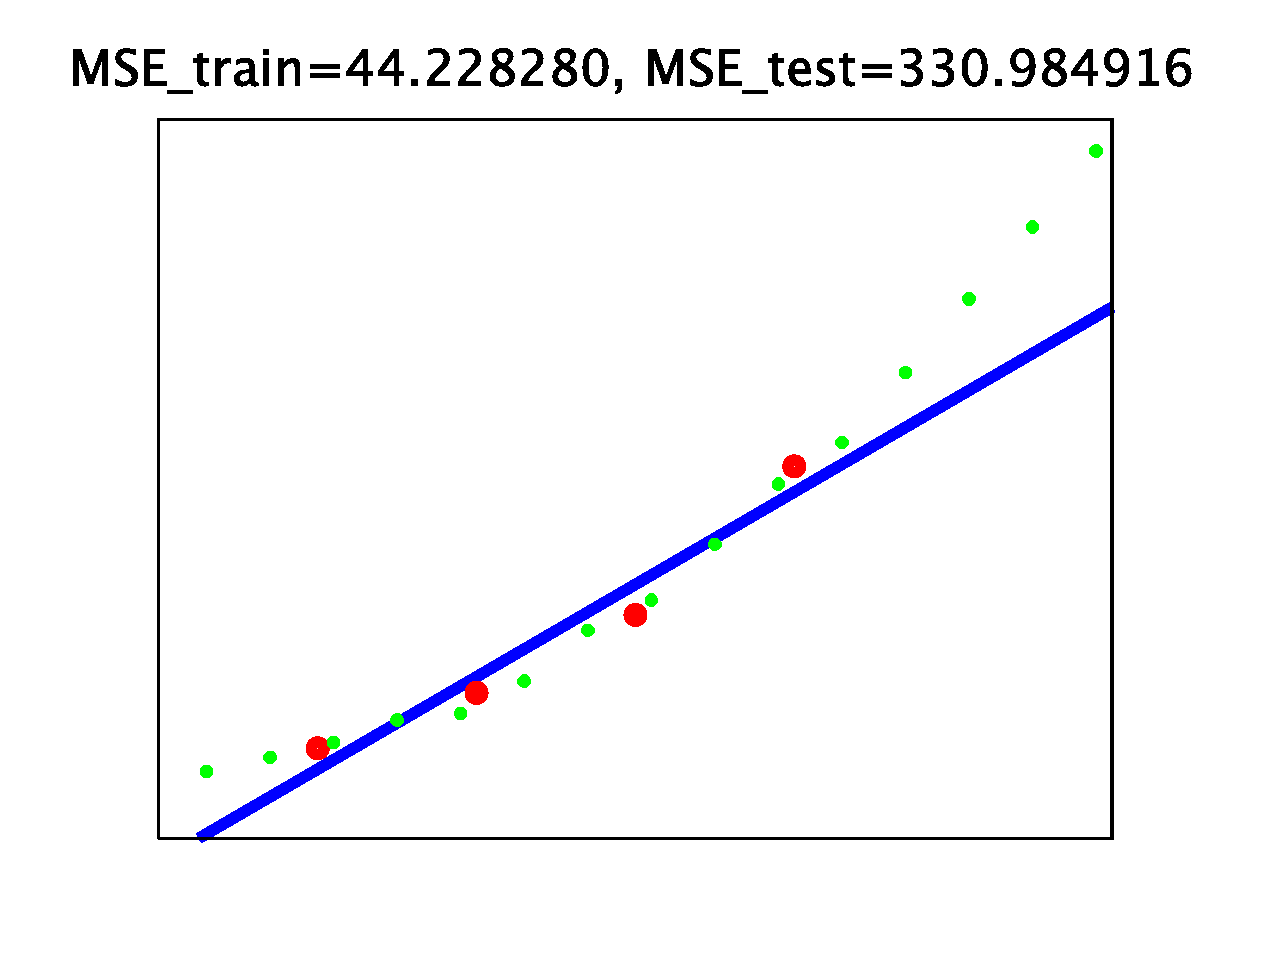
\includegraphics[width=.5\textwidth]{../Figures/linear_regression.pdf}}
\subfigure[Quadratic]{\label{fig:quadratic_regression}
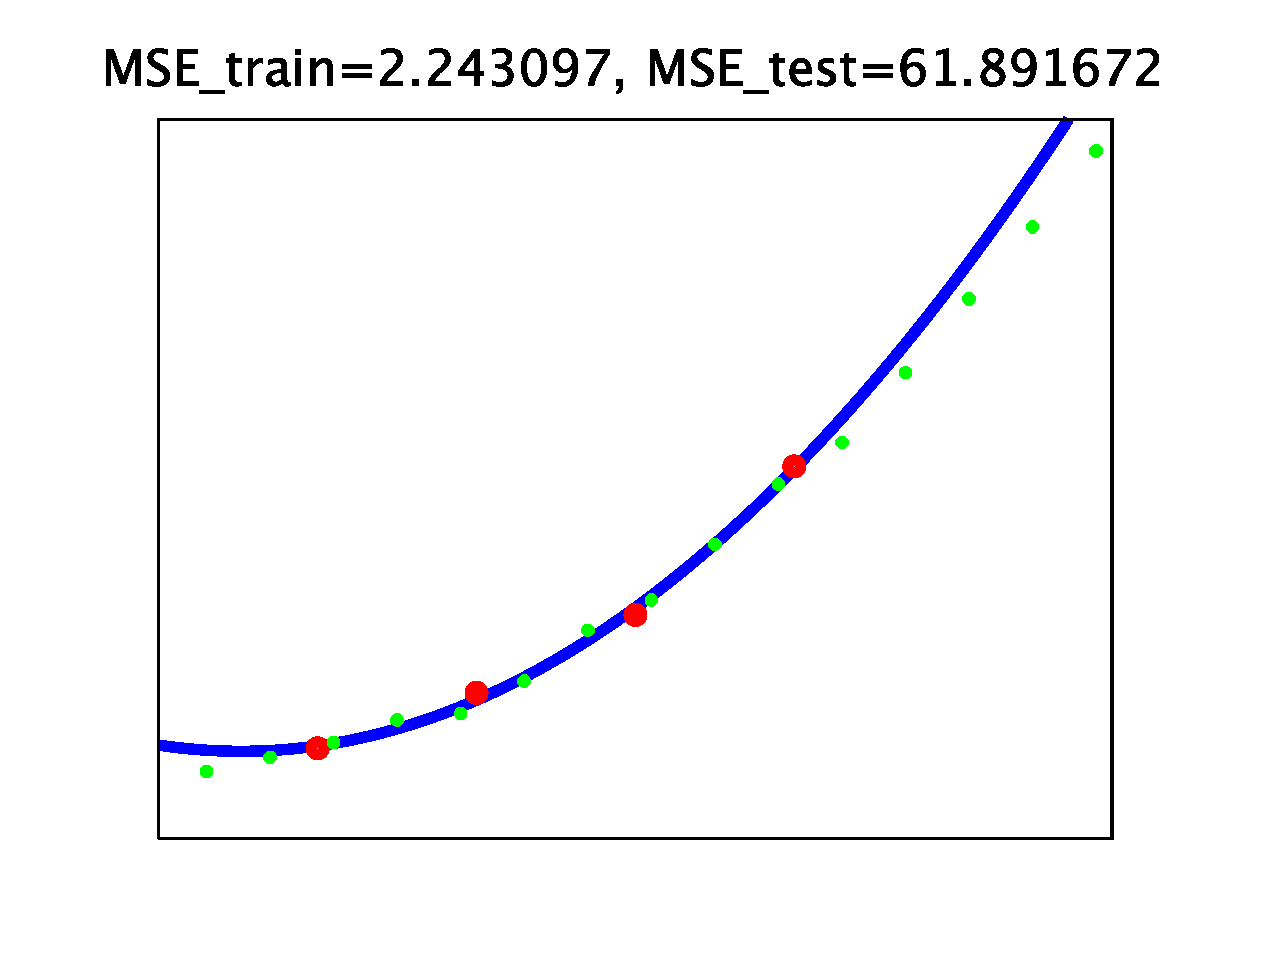
\includegraphics[width=.5\textwidth]{../Figures/quadratic_regression.pdf}}
\subfigure[Cubic]{\label{fig:cubic_regression}
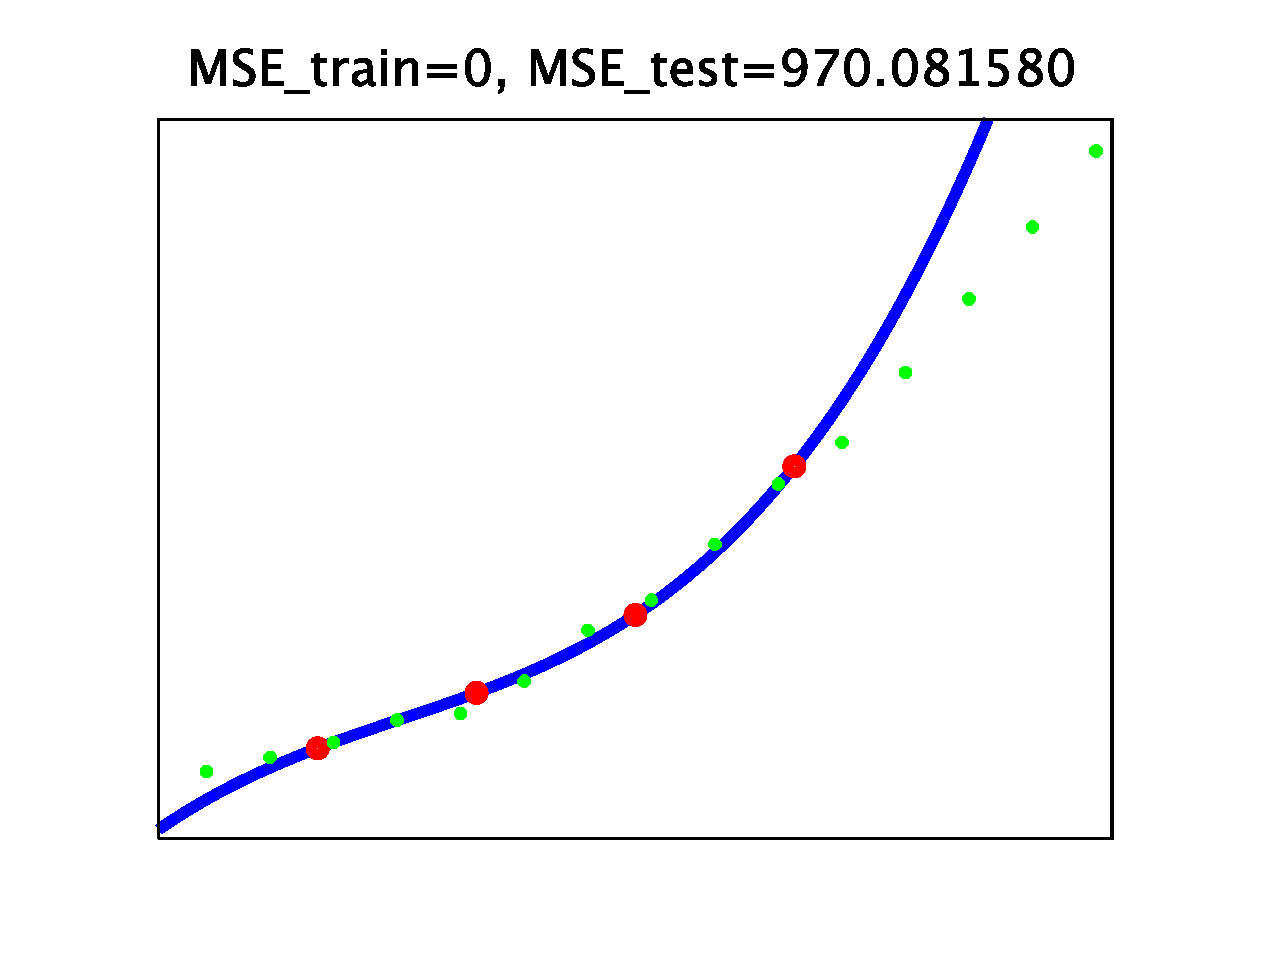
\includegraphics[width=.5\textwidth]{../Figures/cubic_regression.pdf}}
\subfigure[Cubic, more training data]{\label{fig:cubic_more_data}
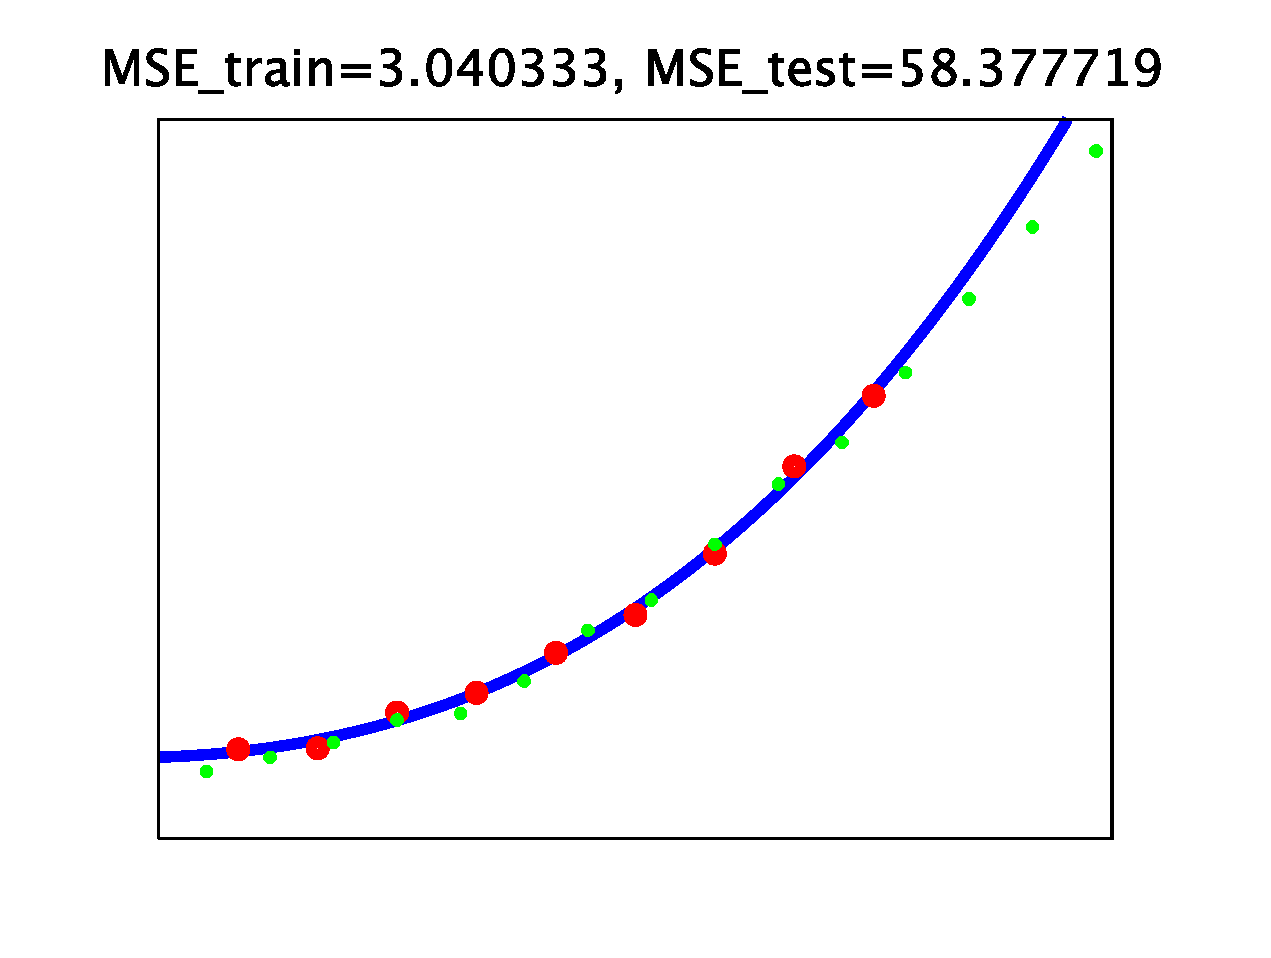
\includegraphics[width=.5\textwidth]{../Figures/cubic_regression_more.pdf}}
\caption[Examples of underfitting and overfitting over a regression problem.]{Examples of underfitting and overfitting over a regression problem. Linear \subref{fig:linear_regression}, quadratic \subref{fig:quadratic_regression} and cubic regression for a truly noised quadratic problem. Red circles are the training examples, green points are the test ones, the blue line represents the learned solution. Linear \subref{fig:linear_regression} regression underfits data, cubic \subref{fig:cubic_regression}  regression overfits data. \subref{fig:cubic_more_data} Cubic regression for a noised quadratic problem and more training examples. The cubic model trained over more data is better adapted to the truly quadratic data, and overfitting is attenuated.}\label{fig:poly_reg}
\end{figure}

\paragraph*{Regularization.}
In a real-case problem, the optimal capacity necessary to learn from given data is unknown. In such a case, trying to fit data with a too low capacity model assures the failure, thus it is always more interesting to oversize the capacity of the learning model. Choosing an oversized model, we risk to incur in overfitting. The so-called \emph{regularization} techniques respond to such a risk, as a widely adopted alternative to DA: in general they consist in adding constraints to the learning algorithm in order to guide it in choosing a model among a wide set of eventually fitting models. Going back to the polynomial regression example, one can try to fit data with a cubic polynomial (thus oversizing the model capacity) and induce the optimiser algorithm to choose the smallest-degree polynomial fitting data via a regularization. This can be obtained adding a penalty that depends on the polynomial degree to the cost function. Applying regularization may make the algorithm be less accurate in learning training data, but more likely to correctly operate on new examples.

\subsection{Hyper-Parameters and Validation}\label{sec:validation}
The \emph{hyper-parameters} of a model are all the parameters that are priorly set and that are not learned by the learning algorithm. They define the general form of the model. In the polynomial regression example the model had a single hyper-parameter: the degree of the polynomial. It is evident from the example that such a parameter is somehow forced not to be optimised by the means of the learning algorithm: trying to reduce the training MSE, the algorithm would choose a sufficient high degree to interpolate all training points (typically $N-1$ if $N$ is the number of training examples). This would cause overfitting, as shown in Fig.~\ref{fig:cubic_regression}. In general among all parameters of a model, the hyper-parameters are chosen as those that can not be learned from data because it would cause overfitting, as in the example, or because they are too difficult to optimise. \\
A way to choose a setting for hyper-parameters consists in performing a \emph{validation} phase. To do so, the training set is split into two disjoint sets, one still called \emph{training set} and the other one called \emph{validation set}. We can say that as the training set is used to learn the parameters, the validation set is used to somehow learn the hyper-parameters. Indeed during or after the training over the training set, the validation set is used to compute a sort of estimation of the test error, which quantifies the generalisation ability of the model. In practice the performances of the (partially) trained model are evaluated over the validation set computing a validation error and hyper-parameters are updated accordingly, in order to reduce the generalisation gap of the model. Once the model has been validated, \ie the hyper-parameters are definitely set, the real test error is evaluated over the test set. Usually the validation error is an underestimation of the test error, since hyper-parameters have been set to reduce it. \\
The validation process just described may strongly depend on the way the training set have been split to create the validation one. In order to avoid to validate a model in a strongly data-dependent way, a slightly different process is encouraged in ML community, named the \emph{cross-validation}, which we describe in Appendix~\ref{app:cross-validation}.


\subsection{No Free Lunch Theorem}\label{sec:NFL}
A so-called \emph{No Free Lunch Theorem} has been formulated for optimisation and ML algorithms around 1997 \cite{wolpert1997no}. It states that any learning algorithm has the same test error if averaged over all possible distributions of data. This means that there cannot exist a universal best ML algorithm: any of them performs in the same way, when performances are averaged over all possible tasks. Thus, making research over some kind of data, for example SCA traces, means trying to understand what kinds of ML algorithms perform well over such particular kind of data and point out the eventual interesting hyper-parameters of ML models that are responsible of the main performance variations. 




%----------------------------------------------------------------------------------------
%	SECTION 3
%----------------------------------------------------------------------------------------
\section{Overview of Machine Learning in Side-Channel Context}
In 1991 Rivest pointed out for the first time a strong link between the fields of Machine Learning and Cryptanalysis \cite{rivest1991cryptography}. Starting from observing that the goal of cryptanalysis is identifying an unknown encryption function, indexed by a secret key, and that a classic problem in ML consists as well in learning an unknown function, he drew a strong correspondence between terminology and concepts of the two fields.\\

In the context of Side-Channel Cryptanalysis, ML algorithms started to be investigated in 2011 \cite{machineLearningSCA}. In this paper the authors formulated for the first time an attack in terms of classification problem and proposed the Support Vector Machine (SVM) \cite{cortes1995support,weston1998multi} as technique to solve it. They also equipped the SVM with a kernel function to allow it to succeed even in case data would not be linearly separable. Such an approach is similar to the one we will describe in Chapter~\ref{ChapterKernel}, to obtain Kernel Discriminant Analysis dimensionality reduction technique from the Linear Discriminant Analysis. Further works analysed the use of SVM in SCA context, proposing concrete attack scenarios \cite{intelligentMachineOmicide,effTA_SVM}. 
The technique of Random Forest \cite{lior2014data} drew attention of the SCA community as well. As the SVM, it has been used as a classifier and has been evaluated in different works \cite{lerman2015machine,lerman2015template,lerman2014power}. As in recent years the privileged tools to tackle classification problem in ML area are the Neural Networks, whose multi-layer configuration has given name to the so-called \emph{Deep Learning} domain, such tools have as well been analysed in SCA context. Networks in the form of Multi-Layer Perceptrons (MLP) have been proposed as classifiers for side-channel traces in a series of works \cite{martinasek2013optimization,martinasek2013innovative,martinasek2015profiling,martinasek2016profiling}, while Convolutional Neural Network was firstly introduced in \cite{maghrebi2016breaking}. A part of this thesis contributions consists in the application of the convolutional paradigm as a way to defeat misalignment countermeasures in side-channel attacks (see Chapter~\ref{ChapterCNN}).

%\subsection{Profiled Attack as a Classification Problem}
%\todo{remark that LDA is first of all a linear method for classification and has been introduced in SCA many years ago as preprocessing for Gaussian TA}
%\subsubsection{Support Vector Machine}
%\subsubsection{Random Forest}
%\subsubsection{Neural Networks}

%\begin{table}[]
%\centering
%\caption{Examples of hyper-parameters}
%\label{tab:hyperparameters}
%\begin{tabular}{c|c}
%\multicolumn{1}{c}{\textbf{Training Hyper-Parameters}} & \multicolumn{1}{c}{\textbf{Architecture Hyper-Parameters}}    \\
%\hline
%training set size                             & number of layers                                     \\
%batch size                                    & nature of each layer{\scriptsize  (\eg FC, ACT,$\dots$)} \\
%number of epochs                              & number of units     \rdelim\}{1}{3mm}[{\scriptsize for FC layers}]                 \\
%optimizer algorithm              &  number of filters               \rdelim\}{4}{3mm}[{\scriptsize for CONV layers}]                          \\
%(initial) learning rate              & kernel size                           \\
%                                              & stride                                               \\
%                                                  & padding                                              \\
%                                              & activation function                  \rdelim\}{1}{3mm}[{\scriptsize for ACT layers}]             \\                   
%                                          
%                                              & pooling function        \rdelim\}{3}{3mm}[{\scriptsize for POOL layers}]                                              \\
%                                              & kernel size \\
%                                              & stride                                              
%\end{tabular}
%\end{table}